\documentclass[aspectratio=169]{beamer}

\usepackage{amsmath,amssymb}
\usepackage{tikz}
\usepackage{graphicx}
\usepackage{multicol}
\usetikzlibrary{angles,quotes} 

\usetheme{Boadilla}
\usecolortheme{orchid}

\newcommand{\justmath}{
  \setbeamercolor{background canvas}{bg=black!15!white}
  \setbeamercolor{block body}{bg=black!30!white}
  \setbeamercolor{block title}{bg=black!85!white}
  \setbeamercolor{frametitle}{fg=black}
  \setbeamercolor{author in head/foot}{bg=black!85!white}
  \setbeamercolor{title in head/foot}{bg=black!70!white}
  \setbeamercolor{date in head/foot}{bg=black!30!white}
}


\title{PHYS 2350: Newton's 2\textsuperscript{nd} Law}
\author{Dr. Wolf}
\date{Fall 2023}

\begin{document}

\begin{frame}
  \titlepage
\end{frame}

%% More Frames as needed
\begin{frame}
  {Newton's Second Law}
  \[
    \vec{F}_{\text{net}} = m\vec{a}
  \]
  \begin{block}
    {What questions are we trying to answer with this equation?}
      \begin{itemize}
        \item Given all of the interactions of outside systems on an object, how is that object
        moving? (Acceleration, velocity, position).  
        \item Given the motion of an object, what are the interactions that cause it to move in
        this way? (Find the net force, or how a specific force interacts with that object given
        other known forces)
      \end{itemize}
  \end{block}
\end{frame}

\begin{frame}
  {Problem type 1:}
  \begin{block}
    {Know the force, find the motion} A block with mass $m$ slides down a inclined plane that
    makes an angle $\theta$ with the horizontal.  What is the magnitude of the acceleration of
    the block as it slides down the ramp? You have consulted a table and found that this
    particular block has a coefficient of kinetic friction of $\mu_k$ with this ramp.
  \end{block}
  Interactions:
  \begin{description}
    \item[Gravity] Force that the earth exerts on the block.  Magnitude: $mg$, direction:
    ``down''
    \item[Normal] Force that the ramp exerts on the block. Magnitude: $N$, direction:
    perpendicular to the surface of the ramp.
    \item[Kinetic Friction] Force that the ramp exerts on the block.  Magnitude $\mu_k N$,
    direction: parallel to the surface of the ramp, going up the ramp.
  \end{description}
\end{frame}

  \begin{frame}
    {Finding the acceleration}
    \begin{columns}
      \begin{column}{0.5\textwidth}
        Draw Free Body diagram:
    
        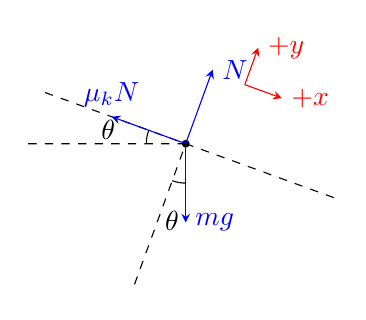
\begin{tikzpicture}[>=stealth]
          \coordinate (O) at (0,0); \coordinate (A) at (-2,0); \coordinate (B) at (0,-2);
          \coordinate (F) at (160:1); \coordinate (P) at (-110:2); \coordinate (G) at (0,-1);
          \draw[dashed] (-20:2) -- (160:2); \draw[dashed] (A) -- (O) -- (P); \fill (O) circle
          (0.05); \draw[->,blue] (O) -- (0,-1) node[right]{$mg$}; \draw[->,blue] (O) -- (70:1)
          node[right]{$N$}; \draw[->,blue] (O) -- (160:1) node[above]{$\mu_k N$}; \draw[->,red]
          (0.75,0.75) -- +(-20:0.5) node[right]{$+x$}; \draw[->,red] (0.75,0.75) -- +(70:0.5)
          node[right]{$+y$};

          \draw pic ["$\theta$",draw,angle eccentricity = 2]{angle=F--O--A}; \draw pic
          ["$\theta$",draw,angle eccentricity = 2]{angle=P--O--G};
        \end{tikzpicture}
        
        Set up equations of motion (Note, acceleration in y-direction is zero)
        \begin{align}
          mg\cos\theta - \mu_k N = ma \\
          N - mg\sin\theta = 0
        \end{align}
        2 equations, 2 unknowns $(N,a)$, let's solve!
      \end{column}
      \begin{column}
        {0.5\textwidth}
        Solve (2) for $N$:
        \[
          N = mg\sin\theta
        \]
        Plug into (1):
        \[
          mg\cos\theta - \mu_k mg\sin\theta = ma
        \]
        Solve for $a$ and win:
        \[
          a = g\left(\cos\theta - \mu_k \sin\theta\right)
        \]
      \end{column}
    \end{columns}
  \end{frame}

\end{document}
